\section{Prioritized-Timed Colored Petri Nets}\label{petrinet}

In this section we introduce the specific model of prioritized-timed
coloured Petri net that we consider for the translation. 
In the
literature on timed extensions of Petri nets we can identify a
first group of models, which assign time delays to transitions,
by using either a fixed deterministic value
\cite{Ram73,Sif77,VFC93} or choosing it from a probability
distribution \cite{AjCh85}. Other models use time intervals to
establish the enabling times of transitions \cite{Mer74}. 
There are also models that introduce time on tokens
\cite{van93,van95,BLT90}. In \cite{Bow96,Wan98} 
a description is given of the different approaches 
to introduce time in Petri nets.
%
Priorities were also introduced in Petri nets to extend the descriptive 
power of the model \cite{Bau96,Best92,Pet81}, usually by
associating priority levels with transitions and modifying the firing
rule to prevent the firing of a transition when another one with
higher priority is enabled. 

We use prioritized-timed coloured Petri nets, 
which are
a prioritized-timed extension of coloured Petri nets \cite{Jensen97},
the well-known model supported by CPN Tools \cite{CPNTools},
developed by the CPN group at the University of Aarhus.
In this model, places have an associated colour set (data types). 
Each token then  has  an attached data value
({\em token colour}),
which belongs to the colour to which the token is
associated. 

We will use timed colours, for which the first component
will be a non-negative integer value, representing the data value,
and the second component will be the token timestamp,
a natural number representing the time at which the 
token will be available.

There is also a discrete global clock that represents
the total time elapsed in the system model. Arcs also have 
an associated inscription ({\em arc expressions}),
constructed using variables, constants, operators
and functions. 
To evaluate an arc expression we need to
bind the variables, which consists of assigning
a value to the variables that appear in the
arc inscription. These values are then used to
select the token colours that must be removed or added when
firing the corresponding transition.

Arc expressions can also have associated time information
both for place-transition and transition-place arcs.
However, only time inscriptions are needed
in output arcs, and even, when all the output arcs
of a transition have the same time inscription,
there is a shorthand notation in CPN Tools
by which this time information is associated with
the transition instead of the output arcs.
This is the specific model that we use 
in our WS-CDL semantics, i.e. we will only
consider these time inscriptions in the transitions.
We will therefore not use any time inscription
in the arcs.

The time inscription associated with a transition 
is used to specify the delay that must be added to the
current value of the global clock for
every token generated by the firing of the transition.

Transitions can also have associated guards, which
are Boolean expressions that can prevent their firing.
Thus, when a transition has a guard, it must evaluate to
true for the binding to be enabled,
otherwise the binding is disabled and 
the transition cannot be fired. 

\begin{definition} (Notation)

The following notation will be used henceforth:

\vspace*{-0.2cm}

\begin{itemize}
%\item $\nnul$ will denote the set of natural numbers,
%$\nat=\{0,1,2,\ldots\}$ and $\Sigma = \nat \times \nat$.
%%
%\item Multisets are defined as functions $C\,:\,X \rightarrow \nnul$,
%providing us with the number of instances of each element $x\in X$.
%As usual, we will enumerate the elements of a multiset $C$ as follows:
%$C = \{ r_1.x_1,\ldots,r_n.x_n \}$, meaning that $C(x_i)=r_i$,
%for all $i=1,\ldots,n$, and $C(x)=0$, for all $x \neq x_i, \, i=1,\ldots,n$.
%
%The set of multisets over a set $X$ will be denoted by ${\cal B}(X)$.
%For any $x \in X$ and $C\in {\cal B}(X)$ we say that $x \in C$
%if and only if $C(x)>0$.
%
%
\item For any $C_1, C_2 \in {\cal B}(X)$, we define:
  %
  \begin{itemize}
  \item $C_1 + C_2 \in {\cal B}(X)$, where $\forall x \in X\,:\,
        (C_1+C_2)(x)= C_1(x) + C_2(x)$.
  %
  \item $C_1 \subseteq C_2$ if and only if $\forall x \in X\,:\,
        C_1(x) \leq C_2(x)$.
  %
  \item If $C_2 \subseteq C_1$ we can define the subtraction 
        $C_1 - C_2 \in {\cal B}(X)$, where $\forall x \in X\,:\,
        (C_1-C_2)(x)= C_1(x) - C_2(x)$.
  \end{itemize}
%
\item For any $C \in {\cal B}(\Sigma)$, 
we define the first projection
$\Pi_1(C) \in {\cal B}(\nnul)$, 
as follows: $\forall n \in \nnul,\,
\Pi_1(C)(n) = \sum_{m\in \nnul} C(n,m)$.
%
\item For any $C \in {\cal B}(\Sigma)$
and $n\in \nnul$ we define the second projection 
$\Pi_2(C,n)$ as the ordered list that consists of the
elements $(m_1,m_2,\ldots,m_{\Pi_1(C)(n)})$,
such that $(n,m_i) \in C$, $\forall i=1,\ldots, \Pi_1(C)(n)$
and $m_i \leq m_{i+1}$,
$\forall i=1,\ldots, \Pi_1(C)(n)-1$.
%
\item For any $C_1,C_2 \in {\cal B}(\Sigma)$, we say that
$C_1 \preceq C_2$ if and only if the following conditions hold:
  %
  \begin{itemize}
  \item $\Pi_1(C_1) \subseteq \Pi_1(C_2)$.
  %
  \item \mbox{$\forall n \in \nnul$}, taking \mbox{$\Pi_2(C_1,n) = (m^1_1,\ldots,
        m^1_{\Pi_1(C_1)(n)})$} and
        \mbox{$\Pi_2(C_2,n) = $} \linebreak
        $(m^2_1,\ldots,m^2_{\Pi_1(C_2)(n)})$,
        we must have  $m^1_i \geq m^2_i$, $\forall i=1,\ldots,
        \Pi_1(C_1)(n)$.
  \end{itemize}
%
%  
These conditions state that for every $n$ the total number of
elements $(n,m)$ (moving $m$) must be lesser in $C_1$ than in $C_2$, and 
for every element $(n,m)$ in $C_1$ there must be a 
corresponding (distinct element) $(n,m')$ in $C_2$, with $m\geq m'$.
%
\item For any $C_1,C_2 \in {\cal B}(\Sigma)$, with $C_1 \preceq C_2$,
we define $C_2 \ominus C_1$ in the following (recursive) way: 
  %
  \begin{itemize}
  \item For $C_1 = \emptyset$ we take $C_2 \ominus C_1 = C_2$.
  %
  \item For $C_1 \neq \emptyset$, let us consider that 

        \noindent $C_2 = \{ r^1_1.(n_1,m^1_1), \ldots,
         r^1_{i_{n_{1}}}.(n_1,m^1_{i_{n_{1}}}),
        \ldots, r^k_1.(n_k,m^k_1),\ldots, r^k_{i_{n_{k}}}.(n_k,m^k_{i_{n_{k}}}) \}$,
        where $n_l \neq n_j$, $\forall l \neq j$, and
        $m^l_j < m^l_{j+1}$, $\forall l=1,\ldots,k$ and $\forall
        j=1,\ldots,i_{n_{l}}$.

        Since $C_1 \preceq C_2$, we can take one element $(n_l,m) \in C_1$, 
        for some $l\in \{1,\ldots,k\}$, as well as the largest index $j$
        for which $m^l_{j} \leq m$. We then define recursively:
       
        \noindent $C_2 \ominus C_1 = %\begin{array}[t]{l}
        (
        \{ r^1_1.(n_1,m^1_1), \ldots, r^1_{i_{n_{1}}}.(n_1,m^1_{i_{n_{1}}}),
        \ldots,
        r^l_1.(n_l,m^l_1), \ldots,(r^l_{j} - 1).(n_l,m^l_j),\\
        \ldots,
        r^l_{i_{n_{l}}}.(n_l,m^l_{i_{n_{l}}}), 
        \ldots, r^k_1.(n_k,m^k_1),\ldots, r^k_{i_{n_{k}}}.(n_k,m^k_{i_{n_{k}}}) \}
        ) 
        \ominus (C_1 - \{ 1.(n_l,m) \})
        %\end{array}
        $.

        %It is immediate that this recursive definition is correct.
        Thus, $C_2 \ominus C_1$ is obtained by removing from $C_2$ 
        elements $(n,m)$ that correspond to elements $(n,m')$ of $C_1$,
        such that $m$ is the largest value with $m\leq m'$.

        % 
        \vspace*{0.12cm}

        For instance, taking $C_1 = \{
             1.(2,3), 1.(2,5), 1.(1,4), 1.(7,6)
        \}$, and $C_2 = $ \linebreak
        $\{
             1.(2,0), 1.(2,1), 1.(2,2), 1.(1,3), 2.(7,6), 3.(3,3)
        \}$ it follows that $C_1 \preceq C_2$. Then,
        $C_2 \ominus C_1= \{
            1.(2,0), 1.(7,6), 3.(3,3)
        \}$.
  \end{itemize} 
\end{itemize}
\end{definition}

\begin{definition} (Prioritised-Timed Colored Petri Nets)\\
We define a prioritized-timed coloured Petri net (PTCPN)
as a tuple $(P,T,A,V,G,E,\lambda,D,\pi)$, where: %\footnote{
%We use the classical notation on Petri nets to denote the
%precondition and postcondition of both places and transitions:
%%
%\[ \forall x \in P\,\cup\,T\,:\,
%\precond{x} = \{ y \,|\, (y,x) \in A\}~~~~~
%   x^{\bullet} = \{ y \,|\, (x,y) \in A\}
%\]
%}:
%%
\begin{itemize}
\item $P$ is a finite set of {\em places}, with colours
in the set $\Sigma$. Thus, in our case, colours 
will be pairs $(n,x)\in \nnul \times \nnul$, where $n$ is
the token value and $x$ its timestamp.
%
\item $T$ is a finite set of {\em transitions} ($P\cap T = \emptyset$).
%
\item $A \subseteq (P\times T)\,\cup\,(T \times P)$ is a
set of directed {\em arcs}.
%
%
\item $V$ is a finite set of {\em typed variables} in $\Sigma$, 
i.e. ${\it Type}(v) \in \Sigma$, for all $v \in V$.
%
%
\item $G\,:\, T \longrightarrow {\it EXPR}_V$ is the
{\em guard function}, which assigns a Boolean
expression
to each transition, i.e. ${\it Type}(G(t))={\it Bool}$. 
%
\item $E\,:\, A \longrightarrow {\it EXPR}_V$ is the
{\em arc expression function}, which assigns an expression
to each arc, such that ${\it Type}(E(a)) = {\cal B}(\nnul \times \{0\})$,
which corresponds to untimed arcs, since, as mentioned above,
we only attach time delays to transitions.
%
%
\item $\lambda$ is the {\em labelling function}, defined
both on places and transitions.
%
%\begin{itemize}
%\item Places are labeled as
%{\em entry places}, {\em exit places}, {\em error places},
%{\em internal places} and {\em variable places},
%which, respectively, correspond to the following labels:
%$\{{\it in, ok, er, i, rv}\}$. In our specific model, a 
%PTCPN will have an only {\em entry place} $p_{\it in}$, 
%such that $\precond{p_{\it in}} = \emptyset$,
%which will be
%initially marked with a single token of color $(0,0)$. 
%There is also
%an only {\em exit place} $p_{\it ok}$, such that
%$p^{\bullet}_{\it ok}=\emptyset$, which will be marked with 
%one token when the system finishes correctly. Each PTCPN
%has also a single {\em error place} $p_{\it er}$,
%such that $p^{\bullet}_{\it er}=\emptyset$, which will become marked
%with one token in the event of a failure. Variable places
%are denoted by $p_{\it rv}$, to mean that they capture the value
%of variable $v$ in role $r$. We will assume that a special value $e$
%is used to denote that the variable has not yet been 
%assigned. Finally, all the remaining places are
%considered as {\em internal}.
%
%\item Transitions are labeled as follows: $\lambda(t)\in L
%\cup \{ \emptyset \} \cup \{ {\it fail} \}$, where
%$L$ is the set of basic activities, defined as follows:
%%
%\[
%    L = \{ {\it time\_out}, 
%           {\it silent}, {\it noaction}(r), {\it assign}(r,v,n),
%           {\it inter}(r_1,r_2,v_1,v_2) \} 
%\]
%%
%\end{itemize}
%
\item $D\,:\,T \longrightarrow \nnul \times \nnul$, which
is the {\em delay function}, which associates a time
interval to each transition. For $D(t)=[d_1,d_2]$,
this means that a uniform probability function will
be used when $t$ is fired to select the specific discrete
delay in that time interval.
%
\item $\pi\,:\,T \longrightarrow \nnul$ is the
{\em priority function}, which assigns a priority level
to each transition. 
\end{itemize}

In this definition, ${\it EXPR}_V$ denotes the
expressions constructed using the variables in $V$,
with the same syntax admitted by CPN Tools.
\end{definition}

\begin{definition} (Markings)\\
Given a PTCPN $N=(P,T,A,V,G,E,\lambda,D,\pi)$,
a marking $M$ is defined as a function
$M\,:\,P \longrightarrow {\cal B}(\Sigma)$,
which assigns a multiset of colours to each place
(which can be empty). 

A timed marking of a PTCPN $N$ is a pair $(M,x)$, where
$M$ is a marking of $N$ and $x$ is the current system time instant.
%
%

Initial markings are those markings for which
the time annotation of every token is $0$,
and all variable places are marked with a single
token $(0,0)$.
A marked prioritized-timed coloured Petri net (MPTCPN)
is then defined as a triple $(N,M,x)$, where
$N$ is a PTCPN, and $(M,x)$ a timed marking of it.
%
\end{definition}

We define the semantics for MPTCPNs in a similar way as in \cite{CPN09}, 
now taking into account that transitions have associated priorities.
We first introduce the notion of {\em binding}, then
the {\em enabling condition} and finally the {\em firing rule}
for MPTCPNs.

\begin{definition} (Bindings)\\
Let $N=(P,T,A,V,G,E,\lambda,D,\pi)$ be a PTCPN.
A {\em binding} of a transition $t \in T$ is a function
$b$ that maps each variable $v \in {\it Var}(t)$
into a value $b(v) \in \Sigma$, where ${\it Var}(t)$
is defined as the set of variables that appear both
in the guard of $t$ and
in the arc expressions of the arcs connected to $t$.
We will denote by $B(t)$ the set of all possible bindings
for $t \in T$. 

Given an expression $e \in {\it EXPR}_V$, we will denote 
by $e\langle b \rangle$ the evaluation of $e$ for the
binding $b$.

A {\em binding element} is then defined as a pair
$(t,b)$, where $t \in T$ and $b \in B(t)$.
The set of all binding elements is denoted by ${\it BE}$.
\end{definition}

\begin{definition}\label{permitidas} (Enabling condition)\\
Let $N=(P,T,A,V,G,E,\lambda,D,\pi)$ be a PTCPN,
and $(M,x)$ a timed marking of it.
We say that a 
binding element $(t,b) \in {\it BE}$
is {\em enabled} at the time instant $x'$ in the timed marking
$(M,x)$ if and
only if the following conditions are fulfilled:

\begin{enumerate}
\item $x' \geq x$.
%
\item $G(t)\langle b \rangle = {\it true}$.
%
\item For all $p \in \precond{t}$,
$E(p,t)\langle b\rangle_{x'} \preceq M(p)$, 
where 
%
$E(p,t)\langle b \rangle_{x'}$ consists of the same
colours as $E(p,t)\langle b \rangle$, but 
replacing their timestamp (which was $0$) by $x'$.
%

the notation $C_{+x}$ is used to represent the
colour multiset obtained from $C$ by delaying its timestamps
by $x$ time units:
%
\[
C_{+x}(n,y) = \left\{
\begin{array}{cl}
C(n,y-x)~~ & {\rm if}\;y \geq  x\\
0        & {\rm otherwise}
\end{array}
\right.
\]
%
\item There is no other binding element $(t',b') \in {\it BE}$
fulfilling the previous conditions  such that $\pi(t') < \pi(t)$.
% INVERTIDAS LAS PRIORIDADES, PARA EVITAR PROBLEMAS,
% AHORA EL CERO ES LA MAXIMA PRIORIDAD.
%
%
\item $x'$ is the smallest time value for which there exists
a binding element $(t,b)$ fulfilling these conditions.
%
\end{enumerate}
%
\end{definition}

\begin{definition} (Firing rule)\\
Let $N=(P,T,A,V,G,E,\lambda,D,\pi)$ be a PTCPN,
$(M,x)$ a timed marking of $N$, and an enabled
binding element $(t,b) \in {\it BE}$ at 
instant $x'$ in the timed marking $(M,x)$.

The firing of $(t,b)$ at instant $x'$ is non-deterministic,
depending on the chosen delay $d \in \nnul$ for the transition.
This delay is randomly selected in the interval given by $D(t)$. 
%This delay is chosen according to a uniform probability distribution. 
Thus, the new timed marking $(M',x')$ is: 
%
\[
  \forall p \in P\,:\,
  M'(p) = M(p) \ominus E(p,t)\langle b \rangle_{x'} + E(t,p)\langle b
 \rangle_{d+x'}
\]
%
\end{definition}

\begin{figure}


\hspace*{1.0cm}
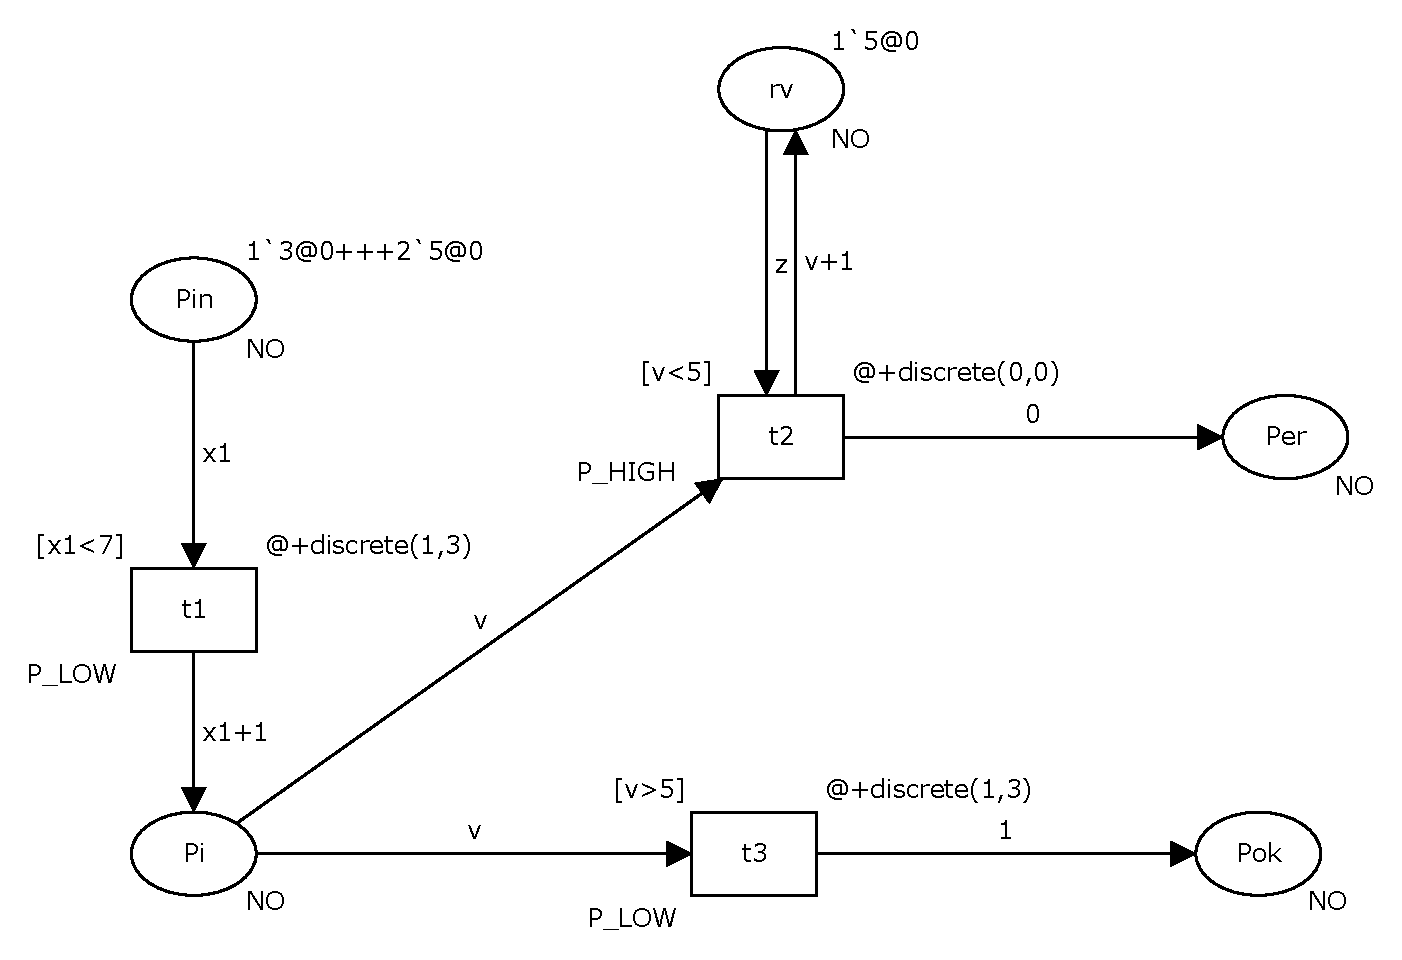
\includegraphics[width=11.5cm]{Figures/figure2_scp.eps}
% 
\caption{\label{red1}Graphical view of a PTCPN.}
\end{figure}


\begin{example} Let us consider the marked PTCPN depicted in Figure \ref{red1}, 
obtained from CPN Tools. 
% 
Observe that timed colour tokens in CPN Tools are drawn
using the notation $n`v@x$,
meaning that we have $n$ instances of a timed colour token 
with colour value $v$ and {\em timestamp} $x$, which correspond to $n.(v,x)$
according to our formal notation. Besides, the symbol `+++'
is there used to represent the union of timed
multisets. 

Thus, $p_{\it in}$ is initially marked with one token
of colour $(3,0)$, and two tokens of colour $(5,0)$,
and the place ${\it rv}$ has one token with colour
$(5,0)$.  Transitions are labeled
with their associated guard, time interval and priority
information. 
Arcs are labeled with the corresponding expressions,
in which no time delays appear, as we are considering
that only transitions have associated time delays.

From the initial marking we can see that
only transition $t_1$ can be fired (at instant $0$), and
any token of those in $p_{\it in}$ can be used for
that purpose.  Taking $(5,0)$ we get the binding $x=5$,
which fulfills the transition guard.
The firing of $t_1$ with this binding removes
one instance of $(5,0)$ from $p_{\it in}$,
and produces a new token on $p_i$.
The timestamp of this new token is a discrete value
in the interval $[1,3]$ (let us say $3$).
Thus, considering the output
arc inscription we get a token $(6,3)$  on $p_i$.

Now, transition $t_1$ must fire again twice (until $p_{\it in}$ 
becomes empty), due to the time constraints of this model. 
As a result we may obtain in $p_i$ the following marking
$\{1.(4,3), 1.(6,1),$
$ 1.(6,3)\}$ (the timestamp values depend on the values
chosen from the interval $[1,3]$).
% 
The only transition that can be fired at this marking
is $t_3$, because due to the time constraints 
we must first use the token $(6,1)$
and $t_2$ cannot be fired using this token.
The firing of $t_3$ produces a new token on $p_{\it ok}$,
whose colour value must be $1$, and the timestamp
depends again on the chosen delay in the time interval
$[1,3]$. For instance, we could obtain the 
colour token $(1,4)$. 

Two tokens now remain in $p_i$, with colours  $(4,3)$ and 
$(6,3)$, and $t_2$ becomes the only transition
enabled (due to condition (4) of Def.\ \ref{permitidas}).
Its firing removes the token $(4,3)$ from $p_i$,
the token on the place ${\it rv}$ changes to $1.(5,3)$,  
and creates a new token on $p_{\it er}$, with colour $(0,3)$. 
%
% 
Finally, the remaining token $(6,3)$ on $p_i$ 
only allows us to fire $t_3$, generating a new token
on $p_{\it ok}$, with value $1$ and a timestamp
depending on the delay chosen for its firing.
\end{example}


In \cite{Buc03} there is a model that
extends Merlin's nets by including dynamic priorities and resources.

The particular model that we use is also an extension of Merlin's
nets, 
% but it is simpler than that considered in \cite{Buc03}.
including priorities and three transition types ({\em black,\,grey\,} and
{\em white\,}). All transitions are assigned both a time interval
and a static priority. The time interval restricts the instants at
which a transition is allowed to be fired. {\em White}\, transitions
are not forced to fire when their clock reaches its latest firing
time, grey transitions must fire once their clock reaches that value, 
and black  transitions
must fire immediately, once they fulfill all the required conditions. 
Of course, in the
event of a conflict, any transition of those involved in the conflict 
can be fired (whichever type it has), although we take into account 
priorities to resolve the conflicts. Thus, priorities are only
used in the case of conflict, when at a given marking two or more
transitions are simultaneously enabled, then only those with 
the maximum priority are allowed to be fired at that moment.

%\begin{definition} (Prioritized-Time Colored Petri Nets)\\
%We define a prioritized-time colored Petri net (PTCPN) as a tuple
%\linebreak $N=(P,\,T,\,F,\alpha,\beta,\pi,\lambda,\Sigma, G)$,
%where\footnote{We use the classical notation on Petri nets to denote the
%precondition and postcondition of both places and transitions:
%%
%\[ \forall x \in P\,\cup\,T\,:\,
%\precond{x} = \{ y \,|\, (y,x) \in F\}~~~~~
%   x^{\bullet} = \{ y \,|\, (x,y) \in F\}
%\] }:
%\begin{itemize}
%  \item $P$ is a finite set of {\em places},  $P= P_i \cup P_c\, 
%        \cup\, \{p_{in}, p_{ok}, p_{er} \}$,
%  where:
%  \begin{itemize}
%    \item $p_{in}$ is the only {\it entry} place of the PTCPN, initially 
%          marked with one
%          token, fulfilling $\,^\bullet p_{in} = \emptyset$.
%%
%    \item $p_{ok}$  is the only {\it exit} place and it will be 
%          marked with one token  when the system
%          finishes correctly, fulfilling $ \, p_{ok}^\bullet = \emptyset$.
%     %
%    \item  $p_{er}$ is the only {\it error} place and it will 
%           become marked with one token in the event of a failure,
%           fulfilling
%           $ \, p_{er}^\bullet = \emptyset $.
%%
%    \item $P_i$:  These are called {\it internal} places, which have
%    precondition and postcondition transitions, $\forall p\in
%    P_i:\quad \,^\bullet p \neq \emptyset \; \vee \; p^\bullet \neq \emptyset
%    $.
%    \item  $P_c$: These are the {\it colored}  places,  labeled with $r_iv_i$,
%    to indicate that they are associated  with  variable
%    $v_i$ of role $r_i$. Their marking will be the corresponding
%    value of $v_i$ in role $r_i$, and initially  they are unassigned
%    (marked with a special value $\epsilon$). For these places $p\in
%    P_c$ we have $^\bullet p= p^\bullet$.
%   \end{itemize}
%
%Markings are defined  as an annotation of tokens over uncolored
%places (they will be represented with black dots), and with the
%value of the variable over the colored places. Hence, a marking $M$
%is formally defined as a function \linebreak \mbox{$M\,:\,P
%\rightarrow \mathbf{Z}\cup\{\epsilon\}$,} where $M(p_k)$ indicates
%the number of tokens on $p_k$, when it is an uncolored place, or it
%indicates the value of the variable $v_i$ (or $\epsilon$ for an
%unassigned variable) for a colored place labeled with $r_iv_i$. We
%will denote by $\mathcal{M}$ the set of all possible markings of a
%Priorized-Time Colored Petri Net.
%
%We consider as  initial marking $M_0$,  the marking in which the
%{\it entry} place is marked with one token, and all the colored
%places are marked with $\epsilon$.
%
%
%\item  $T$ is a finite set of {\em
%transitions}\, ($P \cap T = \emptyset$), such that
%$T=T_w\,\cup\,T_g\,\cup T_b$, which are pairwise disjoint.
%Transitions in $T_w$ are called {\em white}\,, transition in $T_g$
%are called grey,  whereas transitions in $T_b$ are called {\em
%black}\,.
%%
%\item $F$ is the {\em flow relation:\,} $F
%\subseteq (P \times T) \cup (T \times P)$.
%%
%\item $\alpha$ and
%$\beta$ define the time intervals that restrict
%the firing of transitions, $\alpha\,:\, T \rightarrow \nnul$,
%$\beta\,:\, T \rightarrow \nnul\,\cup\,\{\infty\}$, fulfilling
%$\alpha(t)\leq
%\beta(t), \forall t \in T$. 
%%
%\item $\pi$ is the {\em priority
%function\,},\; $\pi\,:\,T \rightarrow \nnul$, which assigns a
%priority level to each transition.
%%
%\item $\lambda: T \rightarrow L \cup \{\emptyset\} \cup \{{\it fail}\}$ is a
%labeling function, where $L$ is the set of basic activities,
%defined as follows: $$ {\it L=\{silent, noaction(r), assign(r,v,n),
%inter(r_1,r_2,v_1,v_2)\}}$$
%%
%\item $\Sigma$ is the set of colors.
%\[ \Sigma \, : \, P_c \rightarrow \mathbf{Z} \cup \{ \epsilon \} \]
%%
%\item $G$ is a guard function $G: T \rightarrow \mathcal{P^M}$ where $\mathcal{P^M}$ are predicates that are obtained by using the markings on the places and the classical logical and arithmetical operators.  We will denote by $G(M,t)$ the evaluation of the predicate of $t$ under marking $M$. We will omit this function in the graphical representation when it is {\it true}.
%\end{itemize}
%%
%\end{definition}
%
%\begin{example} \label{ex1} In Figure \ref{example1} we can see the graphical
%representation of a PTCPN. Transitions are painted in black, grey
%and white according to their type. In Table \ref{tabla_ex} we
%indicate the guards, priorities and the static time intervals that
%the transitions  have associated.  \end{example}
%
%
%The semantics of PTCPNs is captured by the following definitions, which
%extend the firing rule of Merlin's nets by considering the priority
%and color information and the three transition types that we have
%introduced.
%
%\begin{definition} (Enabling transitions)\\
%Given a PTCPN $N=(P,T,F,\alpha,\beta,\pi,\lambda,\Sigma, G)$, a
%marking $M$ of it and a transition $t \in T$, we say that $t$ is
%{\em enabled at $M$\,} if each of its input (uncolored) places
%contains at least one token, i.e. $\forall p \in \precond{t},\,
%p\not\in P_c\,,\, M(p)>0$, i.e. it is enabled in the underlying
%Petri net $(P,T,F)$\footnote{Notice that colored places always have
%one colored token.}. As usual, we denote this by $M[t\rangle$\, and
%the set of transitions enabled at $M$ by $E(N,M)$\,. \end{definition}
%
%We restrict our attention to a particular class of PTCPNs, for which
%no transition will be enabled more that once at a time, i.e. it
%will never be the case that two or more instances of the same
%transition are enabled at a certain instant. With this restriction
%we avoid the semantic problems that appear in Merlin's nets when
%multiple enabling of transitions are allowed (see \cite{Wan98}).
%
%\begin{example}\label{ex2} In the PTCPN of Fig. \ref{example1}, if we consider
%the marking $M$, where $M(p_2)=1$, $M(p_7)=1$, $M(r_1v_1)=1$,
%$M(r_2v_2)=\varepsilon$,  and the remaining places  unmarked, then, we
%have an only  enabled transition, $t_3$.
%\end{example}
%
%\begin{definition} (States in PTCPNs)\\
%Given a PTCPN $N=(P,T,F,\alpha,\beta,\pi,\lambda,\Sigma, G)$, we
%define a {\em state}\, of it
%as a pair $(M,I)$, where $M$ is a marking and $I$ is a %partial
%function $\,\,I\,:\, E(N,M) \rightarrow \nnul \times ( \mathbb{Z }
%\,\cup\,\{\infty\})$, which is defined for enabled transitions, and
%indicates the lower and upper time bounds that they have to be fired
%with respect to the current instant.
%
%For $I(t)=(x_1,x_2)$, we will denote $x_i$ by $\Pi_i(I(t))$, for
%$i=1,2$.
%
%The {\em initial state}\, of a PTCPN is defined by considering an
%initial marking $M_0$ and the function $I_0$ defined by $I_0(t) =
%% \left \{ \begin{array}{ll}
% (\alpha(t),\beta(t))\,, \; \forall t \in E(N,M_0).
%%(\alpha(t),\alpha(t)) \,    & \quad \forall t \in E(N,M_0) \cap T_b
%%\,
%%%
%%\end{array}\right..
%$
%\end{definition}
%
%\begin{example}\label{ex3} For the PTCPN of Fig. \ref{example1}, taking the
%marking $M$ of  Example \ref{ex2}, its initial  state is
%\quad \(I(t_3)=(2,5)\).
%\end{example}
%
%The firing rule can now be precisely defined, but we first need a
%function capturing time elapsing.
%
%\begin{definition} (Time elapsing)\\
%Given a PTCPN $N=(P,T,F,\alpha,\beta,\pi,\lambda,\Sigma, G)$ and a
%state of it $(M,I)$, we say that $x$ units of time can elapse if
%either:
%\begin{itemize}
%\item  $E(N,M)\,\cap\,(T_b\,\cup\, T_g)=\emptyset$, or
%\item  $\forall t \in E(N,M)\,\cap\,(T_b\,\cup\, T_g)$, $G(M,t) \equiv\, false$, or
%\item $\forall t \in  E(N,M)\,\cap\,T_g$, $G(M,t) \equiv\, true$ and  $\Pi_2(I(t)) \geq x$.
%\item $\forall t \in  E(N,M)\,\cap\,T_b$, $G(M,t) \equiv\, true$ and  $\Pi_1(I(t)) \geq x$.
% \end{itemize}
%%
%%
%In that case, the new state reached after that time will be
%$(M,I')$, where
%%
%\[ \forall t \in E(N,M):
%I'(t) = (x_1\menos x, x_2-x) \]
%%
%taking $I(t)=(x_1, x_2)$ and $x
%\menos y = {\it Max} \{0, x - y\}$.
%\end{definition}
%
%From this definition we can see that {\em white\,} transitions may
%lose their opportunity to fire, if they are not fired when their
%clock has reached the latest firing time. This does not mean that
%they are definitely dead, because the tokens on their preconditions
%can be used to fire other transitions, and they can become enabled
%again later. Besides, grey transitions correspond to  Merlin's
%transitions, in the sense that time cannot elapse once the local
%clock of some enabled grey transition whose guard is true reaches
%its latest firing time. For black transitions we impose the
%condition that time cannot elapse once at least one of them is
%enabled, its guard is true and its local clock has reached the
%earliest firing time. Thus, our purpose is that black transitions
%must be fired immediately, once all the required conditions for that
%are fulfilled (unless they are involved in a conflict).
%
%\begin{example}\label{ex4} For the PTCPN of Fig. \ref{example1}, taking again
%the marking $M$ of  \mbox{Example \ref{ex2},} starting  from the
%initial state\; \(I(t_3)=(2,5)\),  $4$ units of time could elapse,
%thus reaching a new state $(M,I')$, with  \(I'(t_3)=(0,1)\).
%%
%\end{example}
%
%The following definition introduces the so-called {\em potentially
%fireable transitions}, which are those that fulfill all the
%required conditions to be fired. However, taking into account
%that a Web Service is a reactive system, only those potentially
%fireable transitions that have been demanded for firing at a given
%instant can actually compete and therefore be fired at that instant.
%For this reason we split the firing into two steps.
%In the first one we consider a set of potentially fireable
%transitions (those that have been demanded), and
%in the second we select from this set the transition
%that is actually fired at that instant (one with the greatest
%priority in this set).
%
%%%%%%%%%%%%%%%%%%%%%%%%%55
%%Definiciones nuevas
%%%%%%%%%%%%%%%%%%%%%%%%%%%%%%%%%%%%55
%\begin{definition}(Potentially Fireable Transitions)\\
%Given a PTCPN $N=(P,T,F,\alpha,\beta,\pi,\lambda,\Sigma, G)$, a
%state $(M,I)$ and an enabled transition $t\in E(N,M)$, we say that
%$t$ is {\it potentially fireable} at that state if and only if the
%following conditions hold:
%\begin{enumerate}
%% Cumple las restricciones de tiempo:
%\item Its associated guard function  is evaluated to true under $M\,$:
%$G(M,t)\equiv\, true.$
%\item\label{condtemp} The earliest firing time of $t$ is 0
%and its latest firing time is greater than or equal to 0\,:
%\,$\Pi_1(I(t))=0\; \wedge \; \Pi_2(I(t)) \geq 0$.
%\end{enumerate}
%\end{definition}
%
%\begin{definition} (Firing rule)\\
%Given a PTCPN $N=(P,T,F,\alpha,\beta,\pi,\lambda,\Sigma, G)$, a
%state of it $(M,I)$, and a set of potentially fireable transitions
%$B$, a transition $t \in B$ {\em can be fired}\, at that state if
%and only if
%there is no other potentially fireable transition in $B$
%having a greater priority:
%$\not\exists t'\in B,\, \, \pi(t')>\pi(t)$.
%
%The firing of $t$ leads us to a new state, $(M',I')$, which is
%defined as follows:
%
%\begin{enumerate}
%\item The marking $M'$ for uncolored places is obtained by applying the classical firing
%rule on Petri nets, i.e. \mbox{$M'(p) = M(p) - W_F(p,t) +
%W_F(t,p)$,} where \mbox{$W_F(a)=1$ for $a\in F$,} and
%\mbox{$W_F(a)=0$} for $a\not\in F$.
%%
%\item The marking of those colored places that are not
%precondition/postcondition of $t$ keep their marking. For
%those colored places $p_c$ (labeled with $r_iv_i$) that are
%precondition/postcondition of $t$ ($p_c \in \,^\bullet t \cap
%t^\bullet$) we change their marking according to the label of $t$.
% For \mbox{$\lambda(t)=$} \mbox{${\it
%asssign}(r_i,v_i,n)$,} we take \mbox{$M'(p_c)=n$;} for
%\mbox{$\lambda(t)={\it inter}(r_j,v_j,r_i,v_i)$}, we take
%\mbox{$M'(p_c)=M(\widetilde{p_c})$,} where $\widetilde{p_c}$ is the
%colored place labeled with $r_jv_j$, and for any other transition
%labeling we also keep the same marking.
%%
%\item For every transition $t' \in E(N,M) \cap E(N,M')$, $t'\neq t$,
%we take $I'(t') = I(t')$.
%%
%\item For every transition $t' \in E(N,M') \setminus E(N,M)$
%we take $I'(t') = (\alpha(t'),\beta(t'))$.
%%
%\item In the event that $t \in E(N,M')$ we take
%$I'(t) = (\alpha(t),\beta(t))$.
%%
%\end{enumerate}
%
%\end{definition}
%
%Notice that firing a transition takes no time to complete, so we
%keep in the new state the time restrictions of the transitions that
%were enabled before the firing and remain enabled after it. It can
%also be the case for the fired transition to become enabled again at
%the new marking, in which case it should be observed 
%that its local clock is reset.
%%
%
%\begin{example}\label{ex5} For the PTCPN of Fig. \ref{example1}, taking the
%marking $M$ of  Example \ref{ex2},  from the state $(M,I')$ with\;
%\(I'(t_3)=(0,1)\),  $t_3$ is the only potentially fireable
%transition.  We can then fire $t_3$, reaching the marking M'\,:
%%
%\[M'(p_3)=1, \; M'(p_7)=1, \; M'(r_1v_1)=1, \; M'(r_2v_2)=\varepsilon ,\]
%and the remaining places unmarked.
%%
%\end{example}


